\documentclass[11pt,a4paper]{article}
\usepackage[margin=22mm]{geometry}
\usepackage[T1]{fontenc}
\usepackage{lmodern}
\usepackage{tabularx,booktabs,hyperref,xcolor,array,xurl}
\usepackage{tikz}
\usetikzlibrary{arrows.meta,positioning,fit,shapes.geometric}
\usepackage{enumitem}
\usepackage{listings}
\hypersetup{colorlinks=true,linkcolor=blue,urlcolor=blue,citecolor=blue}
\setlength{\parindent}{0pt}\sloppy
\setlength{\parskip}{6pt}
\renewcommand{\arraystretch}{1.15}
\newcolumntype{Y}{>{\raggedright\arraybackslash}X}
\newcolumntype{P}[1]{>{\raggedright\arraybackslash}p{#1}}
\newcommand{\code}[1]{\nolinkurl{#1}}
\newcommand{\status}[1]{\textbf{#1}}
\lstset{basicstyle=\ttfamily\small,columns=fullflexible,frame=single,framerule=0.4pt,xleftmargin=4pt,showstringspaces=false}
\title{}
\author{}
\date{}

\begin{document}
\begin{center}
{\Large\textbf{23CSE455 Design Patterns}}\\[4pt]
{\LARGE\textbf{Part 3 Findings: Cross-Language Comparison}}\\[6pt]
{\large Design Pattern Identification and Evolution in a Spring MVC-Based Warehouse Management Application}
\end{center}

\textbf{Team: B9}\\
\textbf{Date: 11 October 2026} (re-audited findings)\\
\textbf{Team working repository:} \href{https://github.com/akdswordguy/Team_B9_DP}{akdswordguy/Team\_B9\_DP}\\
\textbf{Companion documents:} \code{report/main.tex} (full report), \code{report/part1_findings.tex}, \code{report/part2_findings.tex}


\begin{tabularx}{\linewidth}{@{}P{0.25\linewidth}P{0.19\linewidth}P{0.10\linewidth}X@{}}
\toprule
Roll number & Student name & Batch \\
\midrule
AM.SC.U4CSE23215 & D Aditya Kiran & CSE C \\
AM.SC.U4CSE23235 & Mithun Krishna & CSE C \\
AM.SC.U4CSE23248 & Sai Kishen K M & CSE C\\
AM.SC.U4CSE23359 & Sivadev Smijith & CSE D \\
\bottomrule
\end{tabularx}

Evidence paths in this document are relative to \code{Team_B9_Findings/Part3-cross-language/} in the team working repository unless stated otherwise.

\section{Selection and traceability}
Part 3 implements the two GoF patterns confirmed in Part 1 in Java, Python, JavaScript and C++:

\begin{tabularx}{\linewidth}{@{}P{0.15\linewidth}YY@{}}
\toprule
Pattern & OpenWMS source it is traced to (Part 1) & What the Part 3 versions do differently\\
\midrule
Observer & \code{EventBroker}, \code{EventDispatcher}, \code{SimpleEventDispatcher}, \code{EventListener}, \code{RootApplicationEvent} at \code{9d263bf} & One \code{EventSubject} interface instead of the broker/dispatcher split; a single subscriber list rather than subscriptions keyed by event class; a concrete \code{RecordingObserver}, which OpenWMS CORE does not contain.\\
Composite & \code{TreeNode<T>}, \code{TreeNodeImpl<T>} at \code{9d263bf} & Separate \code{Container} and \code{Leaf} classes instead of one class with a leaf state, and a recursive \code{traverse} operation, which \code{TreeNode} lacks.\\
\bottomrule
\end{tabularx}

The eight implementations are independent reference implementations of the pattern concepts. They are not copies of the OpenWMS classes and do not modify OpenWMS. Each uses only its language's standard library.

\section{Common specification}
\textbf{Observer.} \code{subscribe}, \code{unsubscribe} and \code{publish} on a subject; an \code{Event} value with a string type; three recording observers. The scenario subscribes all three, publishes \code{STOCK_LOW}, unsubscribes observer 2, then publishes \code{STOCK_REPLENISHED}. The second event must reach observers 1 and 3 only, and event values must be preserved.

\textbf{Composite.} A shared component contract (\code{getName}, \code{addChild}, \code{removeChild}, \code{getChildren}, \code{traverse}) implemented by \code{Container} and \code{Leaf}. The hierarchy is:

\begin{center}
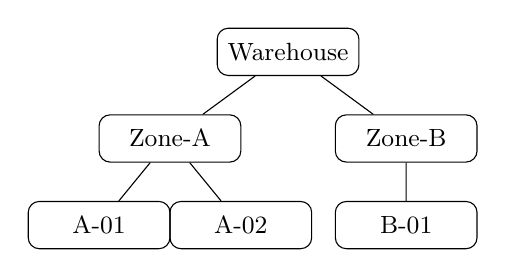
\begin{tikzpicture}[
  level distance=11mm, sibling distance=30mm,
  every node/.style={draw,rounded corners,font=\small,minimum width=18mm,minimum height=6mm},
  level 2/.style={sibling distance=18mm}
]
\node {Warehouse}
  child {node {Zone-A} child {node {A-01}} child {node {A-02}}}
  child {node {Zone-B} child {node {B-01}}};
\end{tikzpicture}
\end{center}
Preorder traversal must return \code{Warehouse, Zone-A, A-01, A-02, Zone-B, B-01}. Leaves return no children and refuse additions.

\section{Implementations and checks}

\subsection{Checks per language}
The same checks exist in every language (names shown in Python/C++ form):

\begin{tabularx}{\linewidth}{@{}P{0.15\linewidth}Y@{}}
\toprule
Pattern & Checks\\
\midrule
Observer (3) & \code{test_all_observers_receive_first_event}; \code{test_unsubscribe_excludes_observer_from_second_event}; \code{test_event_values_and_object_are_preserved} (C++: \code{test_event_values_are_preserved})\\
Composite (4) & \code{test_hierarchy_can_be_constructed}; \code{test_children_can_be_added_and_removed}; \code{test_leaf_rejects_children}; \code{test_recursive_traversal_order}\\
\bottomrule
\end{tabularx}

Java and C++ use executable assertion harnesses (\code{ObserverPatternTest}, \code{observer_test.cpp}, and so on), Python uses \code{unittest}, and JavaScript uses Node's built-in \code{node:assert/strict}. Reporting formats therefore differ, but the scenarios and assertions are equivalent.

\subsection{Results}
\begin{tabularx}{\linewidth}{@{}lYYYY@{}}
\toprule
Pattern & Java & Python & JavaScript & C++\\
\midrule
Observer & 3/3 & 3/3 & 3/3 & 3/3\\
Composite & 4/4 & 4/4 & 4/4 & 4/4\\
\bottomrule
\end{tabularx}

Total 28/28 checks. The results were obtained twice on different machines and toolchains:

\begin{tabularx}{\linewidth}{@{}P{0.20\linewidth}YY@{}}
\toprule
Run & Toolchain & Result\\
\midrule
Recorded run (Windows) & OpenJDK 25.0.4.1 (Temurin), Python 3.13.15, Node.js 24.21.0, g++ 16.2.0 (C++20) & 28/28\\
Re-audit, 11 Oct 2026 (Linux) & OpenJDK 21.0.12.1, Python 3.13.16, Node.js 22.22.0, g++ 13.3.0 (\code{-std=c++20 -Wall -Wextra -Werror -pedantic}) & 28/28\\
\bottomrule
\end{tabularx}

Per-harness console logs were not retained in the repository; the exact commands are in \code{PART3_EVIDENCE.md}.

\section{Static metrics}
LOC is physical lines including blanks and comments. Maximum cyclomatic complexity (CCN) is from Lizard 1.24.1 over both files in each directory. Every value below was recomputed in the re-audit and matches \code{metrics/cross_language.csv}.

\begin{tabularx}{\linewidth}{@{}llrrrrY@{}}
\toprule
Pattern & Language & Impl.\ & Test & Total & Max CCN & Function(s) at max\\
\midrule
Observer & Java & 65 & 70 & 135 & 2 & \code{Publisher.publish}, \code{Publisher.subscribe}, \code{check}\\
Observer & Python & 52 & 37 & 89 & 3 & \code{setUp}, \code{test_event_values_and_object_are_preserved}\\
Observer & JavaScript & 54 & 43 & 97 & 2 & \code{Publisher.subscribe}, \code{Publisher.publish}\\
Observer & C++ & 55 & 61 & 116 & 2 & \code{Publisher::publish}, \code{Publisher::subscribe}, one test\\
Composite & Java & 89 & 63 & 152 & 2 & \code{Container.traverse}, \code{check}, one test\\
Composite & Python & 71 & 48 & 119 & 2 & \code{Container.remove_child}, \code{Container.traverse}\\
Composite & JavaScript & 81 & 47 & 128 & 2 & \code{Container.removeChild}\\
Composite & C++ & 85 & 62 & 147 & 2 & \code{Container::removeChild}, \code{Container::traverse}, one test\\
\bottomrule
\end{tabularx}

\textbf{Structure} (\code{metrics/pattern_metrics.csv}). Every Observer version has 5 named types (3 concrete including the \code{Event} value, 2 abstract contracts), inheritance depth 1 and 3 direct dependency edges; the C++ \code{Event} is a struct. Every Composite version has 3 named types (2 concrete, 1 abstract), inheritance depth 1 and one dependency edge (container to component). Algorithmically, subscribe/unsubscribe and publish are linear in the number of subscribers, traversal is $O(V+E)$, and child add/remove are linear in the number of children.

\section{Dynamic metrics}
Each harness was run as a separate process: one untimed warm-up and 30 timed runs, measured from process launch to exit with the same PowerShell stopwatch; Java and C++ compilation was excluded. Values are the recorded medians from \code{metrics/cross_language.csv} and were not re-measured in the re-audit.

\begin{tabularx}{\linewidth}{@{}lYrr@{}}
\toprule
Pattern & Language & Median process time (ms) & Runs\\
\midrule
Observer & Java & 175.1 & 30\\
Observer & Python & 279.3 & 30\\
Observer & JavaScript & 128.6 & 30\\
Observer & C++ & 33.1 & 30\\
Composite & Java & 154.0 & 30\\
Composite & Python & 264.6 & 30\\
Composite & JavaScript & 130.2 & 30\\
Composite & C++ & 33.4 & 30\\
\bottomrule
\end{tabularx}

These programs do microseconds of real work, so the times are almost entirely runtime start-up (JVM, Python interpreter, Node, or a native executable). They show start-up cost, not the cost of the patterns, and do not support a language-performance ranking.

\section{Comparison}

\subsection{How each language expresses the contracts}
\begin{tabularx}{\linewidth}{@{}P{0.14\linewidth}YYY@{}}
\toprule
Language & Contract mechanism & Observer storage & Composite children\\
\midrule
Java & \code{interface} & \code{ArrayList<Observer>} & \code{List<Component>}, immutable snapshot from \code{getChildren}\\
Python & \code{abc.ABC} with abstract methods & \code{list}, iterated as a \code{tuple} copy & \code{list}, returned as a \code{tuple} snapshot\\
JavaScript & Base class whose methods throw until overridden & private \texttt{\#observers} array & array, shallow copy from \code{getChildren}\\
C++ & Pure virtual class & \code{std::vector<Observer*>} (non-owning) & \code{std::vector<std::shared_ptr<Component>>}\\
\bottomrule
\end{tabularx}

\subsection{Observer}
The subject depends only on the observer contract, so new observers can be added without changing it. All four versions ignore duplicate subscriptions and notify from a copy of the subscriber list, so an observer can unsubscribe during notification safely, as in Python:

\begin{lstlisting}[language=Python]
def publish(self, event: Event) -> None:
    for observer in tuple(self._observers):
        observer.update(event)
\end{lstlisting}

OpenWMS's \code{SimpleEventDispatcher} solves the same problem with a concurrent set per event class, and it also supports subscription by Spring bean name. The C++ version stores raw pointers, so a subscribed observer must outlive its registration; the other three use managed references.

\subsection{Composite}
Clients call \code{getName}, child operations, \code{getChildren} and \code{traverse} without checking the concrete type. \code{Container.traverse} returns its own name and then recurses into each child, which gives preorder. Separating \code{Leaf} from \code{Container} lets a leaf reject \code{addChild} explicitly; OpenWMS's single \code{TreeNodeImpl} instead lets any node gain children.

\subsection{Language observations}
\begin{enumerate}[leftmargin=*,nosep]
\item \textbf{Type system.} Java and C++ check contracts at compile time; Python ABCs enforce abstract methods at instantiation; JavaScript relies on convention and runtime errors.
\item \textbf{Boilerplate.} Python is shortest. The C++ and Java totals are inflated by explicit types and harness code, and LOC is not normalized for formatting.
\item \textbf{Ownership.} Only C++ makes ownership explicit: \code{shared_ptr} for Composite children and non-owning pointers for observers.
\item \textbf{Complexity.} Maximum CCN is 2 to 3 everywhere. That reflects how small the examples are, not design quality.
\end{enumerate}

\section{Limitations}
\begin{itemize}[nosep]
\item These are teaching-sized reference implementations, not production event or location subsystems, and they do not modify OpenWMS.
\item LOC is physical lines; CCN depends on Lizard 1.24.1's parsers for each language.
\item Timings are dominated by process start-up and were measured once on one machine.
\item Raw console logs from the recorded run were not retained.
\end{itemize}

\section{Re-audit summary}
No incorrect values were found in Part 3. All eight harnesses passed again on a second toolchain, and all sixteen file LOC values and eight CCN values were recomputed and match. The only additions are the re-run record in \code{PART3_EVIDENCE.md}, the AUDIT-01 entry in \code{metrics/llm_records.csv} and \code{LLM_RECORDS.md}, and the comparison with the OpenWMS originals in Sections~1 and~6.

\section{Evidence files}
\begin{itemize}[nosep]
\item \code{observer/\{java,python,javascript,cpp\}/} and \code{composite/\{java,python,javascript,cpp\}/} --- implementation and test source.
\item \code{PART3_EVIDENCE.md} --- specification, commands, results, metrics, comparison, re-run record.
\item \code{metrics/cross_language.csv} (8 rows, 19 columns), \code{metrics/pattern_metrics.csv}, \code{metrics/llm_records.csv}.
\item \code{Team_B9_Findings/LLM_RECORDS/LLM_RECORDS.md} --- records P3-01, P3-02 and AUDIT-01.
\end{itemize}

\end{document}
